% Options for packages loaded elsewhere
\PassOptionsToPackage{unicode}{hyperref}
\PassOptionsToPackage{hyphens}{url}
\PassOptionsToPackage{dvipsnames,svgnames,x11names}{xcolor}
%
\documentclass[
  11pt,
  a4paper,
  DIV=11,
  numbers=noendperiod]{scrartcl}

\usepackage{amsmath,amssymb}
\usepackage{iftex}
\ifPDFTeX
  \usepackage[T1]{fontenc}
  \usepackage[utf8]{inputenc}
  \usepackage{textcomp} % provide euro and other symbols
\else % if luatex or xetex
  \usepackage{unicode-math}
  \defaultfontfeatures{Scale=MatchLowercase}
  \defaultfontfeatures[\rmfamily]{Ligatures=TeX,Scale=1}
\fi
\usepackage{lmodern}
\ifPDFTeX\else  
    % xetex/luatex font selection
  \setmainfont[]{Avenir Next}
\fi
% Use upquote if available, for straight quotes in verbatim environments
\IfFileExists{upquote.sty}{\usepackage{upquote}}{}
\IfFileExists{microtype.sty}{% use microtype if available
  \usepackage[]{microtype}
  \UseMicrotypeSet[protrusion]{basicmath} % disable protrusion for tt fonts
}{}
\makeatletter
\@ifundefined{KOMAClassName}{% if non-KOMA class
  \IfFileExists{parskip.sty}{%
    \usepackage{parskip}
  }{% else
    \setlength{\parindent}{0pt}
    \setlength{\parskip}{6pt plus 2pt minus 1pt}}
}{% if KOMA class
  \KOMAoptions{parskip=half}}
\makeatother
\usepackage{xcolor}
\setlength{\emergencystretch}{3em} % prevent overfull lines
\setcounter{secnumdepth}{-\maxdimen} % remove section numbering
% Make \paragraph and \subparagraph free-standing
\ifx\paragraph\undefined\else
  \let\oldparagraph\paragraph
  \renewcommand{\paragraph}[1]{\oldparagraph{#1}\mbox{}}
\fi
\ifx\subparagraph\undefined\else
  \let\oldsubparagraph\subparagraph
  \renewcommand{\subparagraph}[1]{\oldsubparagraph{#1}\mbox{}}
\fi


\providecommand{\tightlist}{%
  \setlength{\itemsep}{0pt}\setlength{\parskip}{0pt}}\usepackage{longtable,booktabs,array}
\usepackage{calc} % for calculating minipage widths
% Correct order of tables after \paragraph or \subparagraph
\usepackage{etoolbox}
\makeatletter
\patchcmd\longtable{\par}{\if@noskipsec\mbox{}\fi\par}{}{}
\makeatother
% Allow footnotes in longtable head/foot
\IfFileExists{footnotehyper.sty}{\usepackage{footnotehyper}}{\usepackage{footnote}}
\makesavenoteenv{longtable}
\usepackage{graphicx}
\makeatletter
\def\maxwidth{\ifdim\Gin@nat@width>\linewidth\linewidth\else\Gin@nat@width\fi}
\def\maxheight{\ifdim\Gin@nat@height>\textheight\textheight\else\Gin@nat@height\fi}
\makeatother
% Scale images if necessary, so that they will not overflow the page
% margins by default, and it is still possible to overwrite the defaults
% using explicit options in \includegraphics[width, height, ...]{}
\setkeys{Gin}{width=\maxwidth,height=\maxheight,keepaspectratio}
% Set default figure placement to htbp
\makeatletter
\def\fps@figure{htbp}
\makeatother

\usepackage[document]{ragged2e}
\KOMAoption{captions}{tableheading}
\makeatletter
\@ifpackageloaded{tcolorbox}{}{\usepackage[skins,breakable]{tcolorbox}}
\@ifpackageloaded{fontawesome5}{}{\usepackage{fontawesome5}}
\definecolor{quarto-callout-color}{HTML}{909090}
\definecolor{quarto-callout-note-color}{HTML}{0758E5}
\definecolor{quarto-callout-important-color}{HTML}{CC1914}
\definecolor{quarto-callout-warning-color}{HTML}{EB9113}
\definecolor{quarto-callout-tip-color}{HTML}{00A047}
\definecolor{quarto-callout-caution-color}{HTML}{FC5300}
\definecolor{quarto-callout-color-frame}{HTML}{acacac}
\definecolor{quarto-callout-note-color-frame}{HTML}{4582ec}
\definecolor{quarto-callout-important-color-frame}{HTML}{d9534f}
\definecolor{quarto-callout-warning-color-frame}{HTML}{f0ad4e}
\definecolor{quarto-callout-tip-color-frame}{HTML}{02b875}
\definecolor{quarto-callout-caution-color-frame}{HTML}{fd7e14}
\makeatother
\makeatletter
\@ifpackageloaded{caption}{}{\usepackage{caption}}
\AtBeginDocument{%
\ifdefined\contentsname
  \renewcommand*\contentsname{Table of contents}
\else
  \newcommand\contentsname{Table of contents}
\fi
\ifdefined\listfigurename
  \renewcommand*\listfigurename{List of Figures}
\else
  \newcommand\listfigurename{List of Figures}
\fi
\ifdefined\listtablename
  \renewcommand*\listtablename{List of Tables}
\else
  \newcommand\listtablename{List of Tables}
\fi
\ifdefined\figurename
  \renewcommand*\figurename{Figure}
\else
  \newcommand\figurename{Figure}
\fi
\ifdefined\tablename
  \renewcommand*\tablename{Table}
\else
  \newcommand\tablename{Table}
\fi
}
\@ifpackageloaded{float}{}{\usepackage{float}}
\floatstyle{ruled}
\@ifundefined{c@chapter}{\newfloat{codelisting}{h}{lop}}{\newfloat{codelisting}{h}{lop}[chapter]}
\floatname{codelisting}{Listing}
\newcommand*\listoflistings{\listof{codelisting}{List of Listings}}
\makeatother
\makeatletter
\makeatother
\makeatletter
\@ifpackageloaded{caption}{}{\usepackage{caption}}
\@ifpackageloaded{subcaption}{}{\usepackage{subcaption}}
\makeatother
\ifLuaTeX
  \usepackage{selnolig}  % disable illegal ligatures
\fi
\usepackage{bookmark}

\IfFileExists{xurl.sty}{\usepackage{xurl}}{} % add URL line breaks if available
\urlstyle{same} % disable monospaced font for URLs
\hypersetup{
  pdftitle={7. Trigonometrische Funktionen},
  colorlinks=true,
  linkcolor={blue},
  filecolor={Maroon},
  citecolor={Blue},
  urlcolor={Blue},
  pdfcreator={LaTeX via pandoc}}

\title{7. Trigonometrische Funktionen}
\author{}
\date{}

\begin{document}
\maketitle

\subsubsection{7.1 Winkelfunktion im
Dreieck}\label{winkelfunktion-im-dreieck}

\paragraph{Rechtwinklige Dreiecke}\label{rechtwinklige-dreiecke}

\textbf{Bezeichnungen in rechtwinklingen Dreiecken}

Allgemein:

\begin{figure}[H]

{\centering 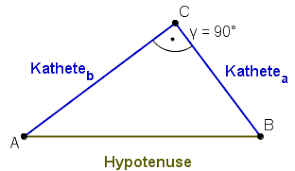
\includegraphics[width=3.125in,height=\textheight]{/Users/martin/Workspace/Jupyter_Notebooks/Mathe_KS/1_Analysis/4_Zusammenhang_Funktion_Graph/images/1rechwinkligesDreieck.png}

}

\caption{Dreieck}

\end{figure}%

Im Bezug auf die Winkel:

\begin{figure}[H]

{\centering 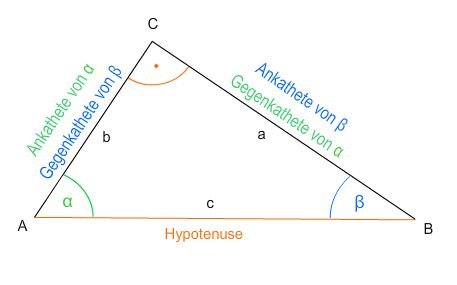
\includegraphics[width=3.125in,height=\textheight]{/Users/martin/Workspace/Jupyter_Notebooks/Mathe_KS/1_Analysis/4_Zusammenhang_Funktion_Graph/images/dreieck_wp.jpg}

}

\caption{Dreieck}

\end{figure}%

\textbf{Beobachtung}

\begin{figure}[H]

{\centering 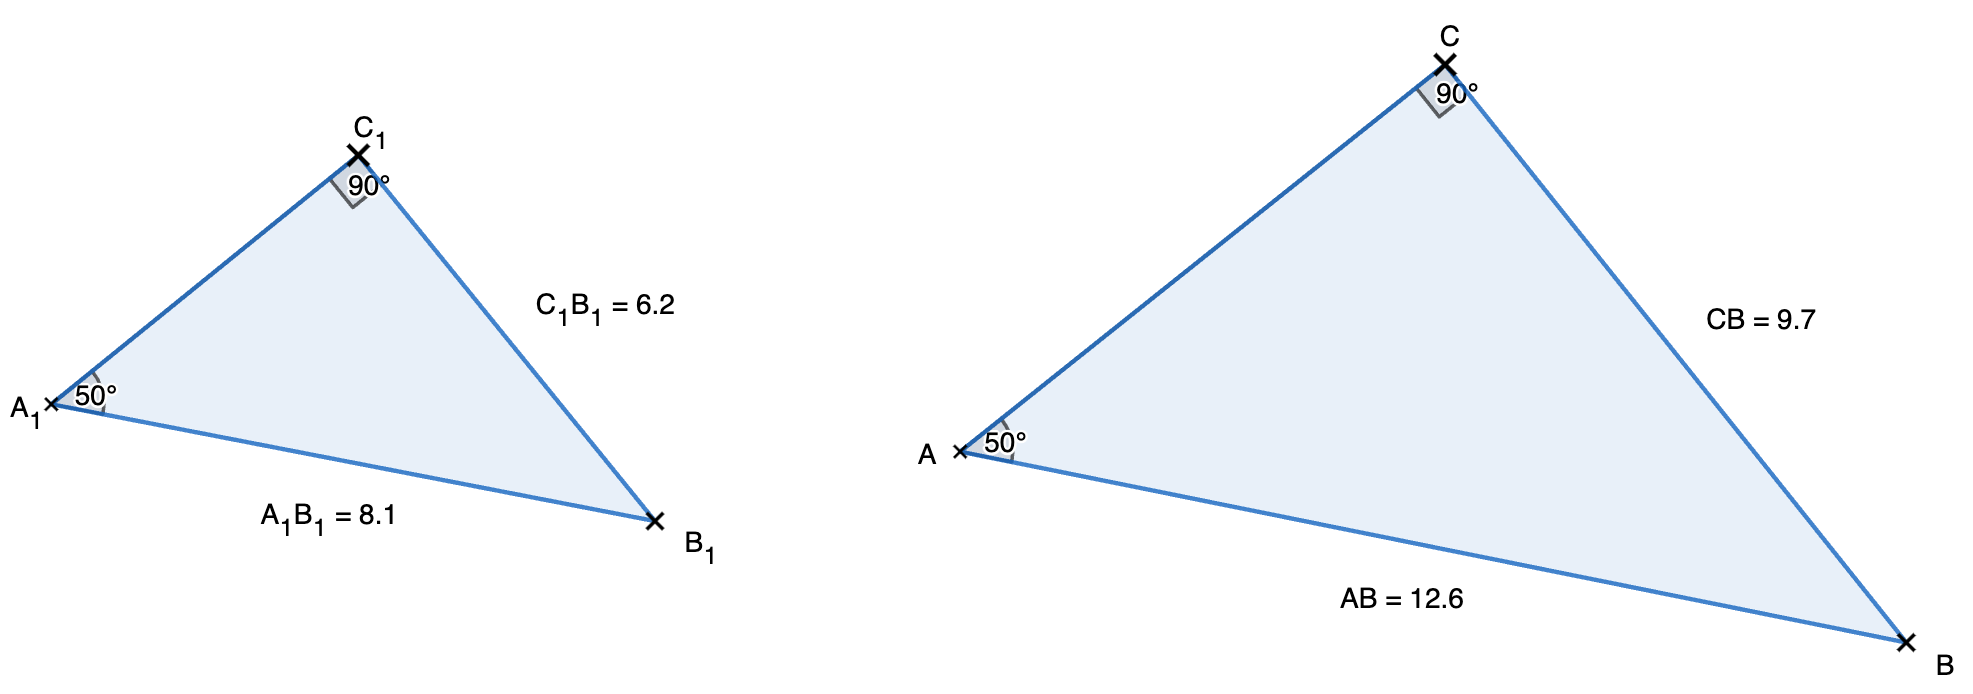
\includegraphics[width=2.08333in,height=\textheight]{/Users/martin/Workspace/Jupyter_Notebooks/Mathe_KS/1_Analysis/4_Zusammenhang_Funktion_Graph/images/2rechtwinkligeDreiecke.png}

}

\caption{Dreieck}

\end{figure}%

\begin{longtable}[]{@{}
  >{\centering\arraybackslash}p{(\columnwidth - 10\tabcolsep) * \real{0.1667}}
  >{\centering\arraybackslash}p{(\columnwidth - 10\tabcolsep) * \real{0.1667}}
  >{\centering\arraybackslash}p{(\columnwidth - 10\tabcolsep) * \real{0.1667}}
  >{\centering\arraybackslash}p{(\columnwidth - 10\tabcolsep) * \real{0.1667}}
  >{\centering\arraybackslash}p{(\columnwidth - 10\tabcolsep) * \real{0.1667}}
  >{\centering\arraybackslash}p{(\columnwidth - 10\tabcolsep) * \real{0.1667}}@{}}
\toprule\noalign{}
\begin{minipage}[b]{\linewidth}\centering
\[ A_1B_1\]
\end{minipage} & \begin{minipage}[b]{\linewidth}\centering
\[ B_1C_1\]
\end{minipage} & \begin{minipage}[b]{\linewidth}\centering
\[ \frac{B_1C_1}{A_1B_1} \]
\end{minipage} & \begin{minipage}[b]{\linewidth}\centering
\[ AB\]
\end{minipage} & \begin{minipage}[b]{\linewidth}\centering
\[ BC\]
\end{minipage} & \begin{minipage}[b]{\linewidth}\centering
\[ \frac{BC}{AB} \]
\end{minipage} \\
\midrule\noalign{}
\endhead
\bottomrule\noalign{}
\endlastfoot
8,1 & 6,2 & 0,76 & 12,6 & 9,7 & 0,76 \\
\end{longtable}

In jedem rechtwinklingen Dreieck mit festem Winkel \(\alpha\) ist das
Verhältnis von Gegenkathete zu \(\alpha\) zur Hypothenuse konstant.
Dieses Verhältnis ist der Sinus zu dem Winkel \(\alpha\)

\textbf{Analog} In jedem rechtwinklingen Dreieck mit festem Winkel
\(\alpha\) ist das Verhältnis von Ankathete zu \(\alpha\) zur
Hypothenuse konstant. Dieses Verhältnis ist der Kosinus zu dem Winkel
\(\alpha\)

\begin{tcolorbox}[enhanced jigsaw, colbacktitle=quarto-callout-note-color!10!white, breakable, bottomtitle=1mm, toptitle=1mm, opacitybacktitle=0.6, opacityback=0, rightrule=.15mm, titlerule=0mm, leftrule=.75mm, colframe=quarto-callout-note-color-frame, toprule=.15mm, left=2mm, colback=white, title=\textcolor{quarto-callout-note-color}{\faInfo}\hspace{0.5em}{Definition: Sinus}, coltitle=black, arc=.35mm, bottomrule=.15mm]

Gegeben:

\begin{itemize}
\tightlist
\item
  rechtwinkliges Dreieck ABC
\item
  Winkel \(\alpha, \beta, \gamma = 90^\circ\)
\end{itemize}

Der Sinus eines Winkels ist das Verhältnis der Länge der Gegenkathete
zur Länge der Hyopthenuse \[
\sin(\alpha) =  \frac{\text{Gegenkathete zu }\alpha}{\text{Hypothenuse}}
\]

\end{tcolorbox}

\begin{tcolorbox}[enhanced jigsaw, colbacktitle=quarto-callout-note-color!10!white, breakable, bottomtitle=1mm, toptitle=1mm, opacitybacktitle=0.6, opacityback=0, rightrule=.15mm, titlerule=0mm, leftrule=.75mm, colframe=quarto-callout-note-color-frame, toprule=.15mm, left=2mm, colback=white, title=\textcolor{quarto-callout-note-color}{\faInfo}\hspace{0.5em}{Definition: Kosinus}, coltitle=black, arc=.35mm, bottomrule=.15mm]

Gegeben:

\begin{itemize}
\tightlist
\item
  rechtwinkliges Dreieck ABC
\item
  Winkel \(\alpha, \beta, \gamma = 90^\circ\)
\end{itemize}

Der Kosinus eines Winkels ist das Verhältnis der Länge der Ankathete zur
Länge der Hypothenuse \[
\cos(\alpha) =  \frac{\text{Ankathete zu }\alpha}{\text{Hypothenuse}}
\]

\end{tcolorbox}

\begin{tcolorbox}[enhanced jigsaw, colbacktitle=quarto-callout-note-color!10!white, breakable, bottomtitle=1mm, toptitle=1mm, opacitybacktitle=0.6, opacityback=0, rightrule=.15mm, titlerule=0mm, leftrule=.75mm, colframe=quarto-callout-note-color-frame, toprule=.15mm, left=2mm, colback=white, title=\textcolor{quarto-callout-note-color}{\faInfo}\hspace{0.5em}{Definition: Tangens}, coltitle=black, arc=.35mm, bottomrule=.15mm]

Gegeben:

\begin{itemize}
\tightlist
\item
  rechtwinkliges Dreieck ABC
\item
  Winkel \(\alpha, \beta, \gamma = 90^\circ\)
\end{itemize}

Der Sinus eines Winkels ist das Verhältnis der Länge der Gegenkathete
zur Länge der Ankathete \[
\tan(\alpha) =  \frac{\text{Gegenkathete zu }\alpha}{\text{Ankathete zu }\alpha}
\]

\end{tcolorbox}

\subparagraph{Sinus, Kosinus und Tangens am
Einheitskreis}\label{sinus-kosinus-und-tangens-am-einheitskreis}

\begin{itemize}
\tightlist
\item
  Einheitskreis := Kreis um den Ursprung mit Radius 1
\item
  Zu jedem Punkt \(P\) auf dem Kreis gibt es ein rechtwinkliges Dreieck
\item
  Länge der Hypothenus ist 1.
\end{itemize}

\begin{figure}[H]

{\centering 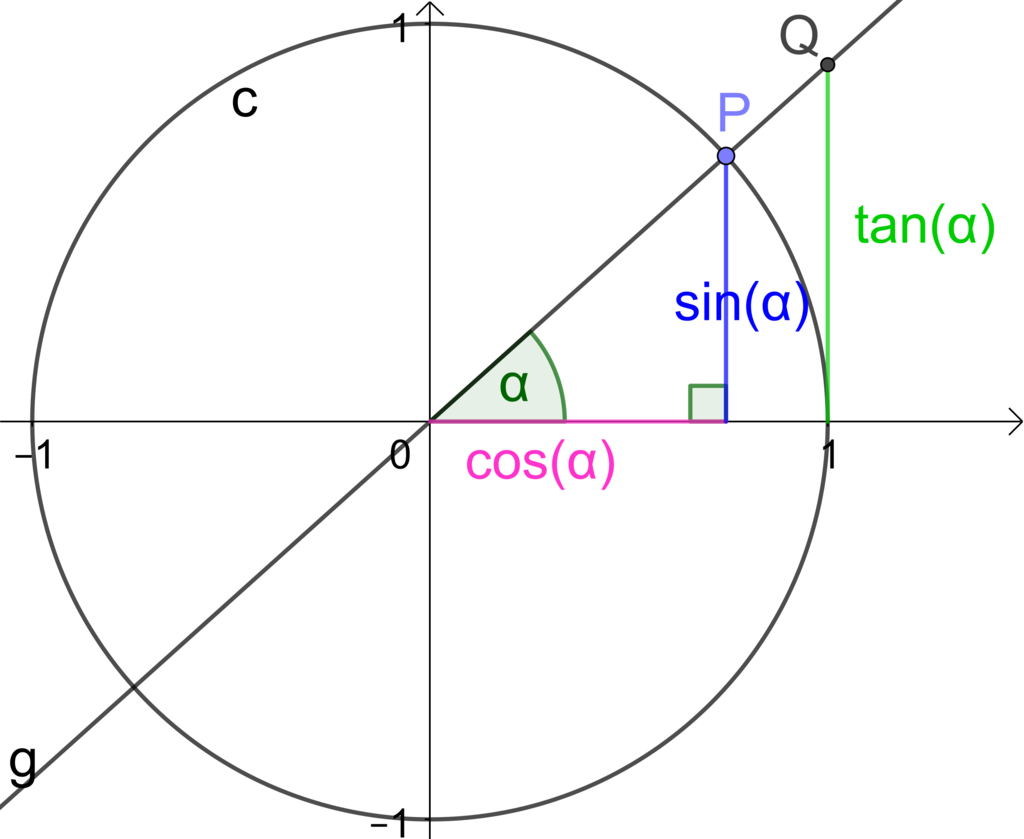
\includegraphics[width=2.60417in,height=\textheight]{/Users/martin/Workspace/Jupyter_Notebooks/Mathe_KS/1_Analysis/4_Zusammenhang_Funktion_Graph/images/4sincostaneinheitskreis.png}

}

\caption{Einheitskreis}

\end{figure}%

\subparagraph{Sinus, Kosiunsfunktion und Tangensfunktion im
Dreieck}\label{sinus-kosiunsfunktion-und-tangensfunktion-im-dreieck}

\begin{figure}[H]

{\centering 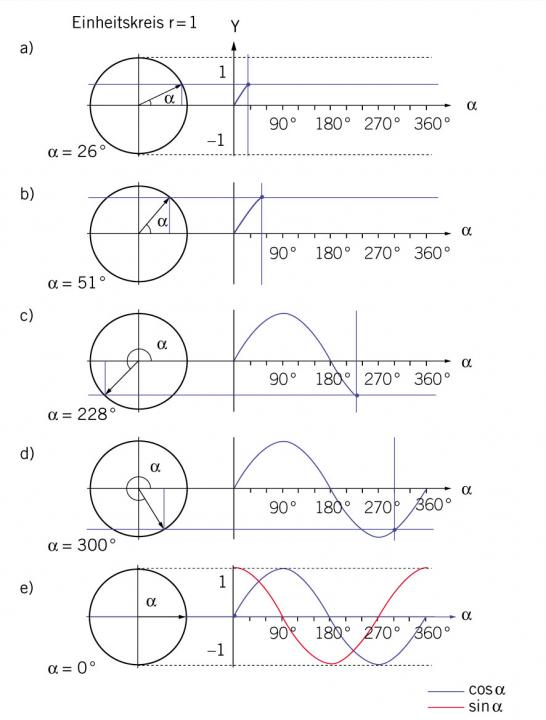
\includegraphics[width=5.20833in,height=\textheight]{/Users/martin/Workspace/Jupyter_Notebooks/Mathe_KS/1_Analysis/4_Zusammenhang_Funktion_Graph/images/5sincosfunktion.jpg}

}

\caption{Sinusfunktion}

\end{figure}%

\begin{tcolorbox}[enhanced jigsaw, colbacktitle=quarto-callout-note-color!10!white, breakable, bottomtitle=1mm, toptitle=1mm, opacitybacktitle=0.6, opacityback=0, rightrule=.15mm, titlerule=0mm, leftrule=.75mm, colframe=quarto-callout-note-color-frame, toprule=.15mm, left=2mm, colback=white, title=\textcolor{quarto-callout-note-color}{\faInfo}\hspace{0.5em}{Definition: Sinusfunktion im Dreieck}, coltitle=black, arc=.35mm, bottomrule=.15mm]

Gegeben:

\begin{itemize}
\tightlist
\item
  rechtwinkliges Dreieck ABC
\end{itemize}

Die Abbildung, die jeder Winkelgröße den Sinus zum Winkel im zugehörigen
rechtwinkligen Dreieck zuordnet, heißt \textbf{Sinusfunktion}

\end{tcolorbox}

\textbf{Funktionsgraph der Sinus-Funktion:}

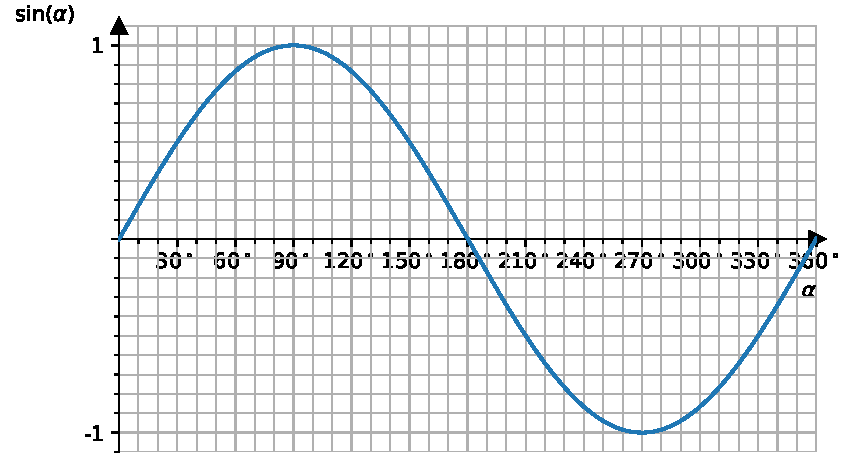
\includegraphics{7_Trigonometrische_Funktionen_files/figure-pdf/cell-2-output-1.pdf}

\begin{tcolorbox}[enhanced jigsaw, colbacktitle=quarto-callout-note-color!10!white, breakable, bottomtitle=1mm, toptitle=1mm, opacitybacktitle=0.6, opacityback=0, rightrule=.15mm, titlerule=0mm, leftrule=.75mm, colframe=quarto-callout-note-color-frame, toprule=.15mm, left=2mm, colback=white, title=\textcolor{quarto-callout-note-color}{\faInfo}\hspace{0.5em}{Definition: Kosinus-Funktion im Dreieck}, coltitle=black, arc=.35mm, bottomrule=.15mm]

Gegeben:

\begin{itemize}
\tightlist
\item
  rechtwinkliges Dreieck ABC
\end{itemize}

Die Abbildung, die jeder Winkelgröße den Kosinus zum Winkel im
zugehörigen rechtwinkligen Dreieck zuordnet, heißt
\textbf{Kosinusfunktion}

\end{tcolorbox}

\textbf{Funktionsgraph der Kosinus-Funktion:}

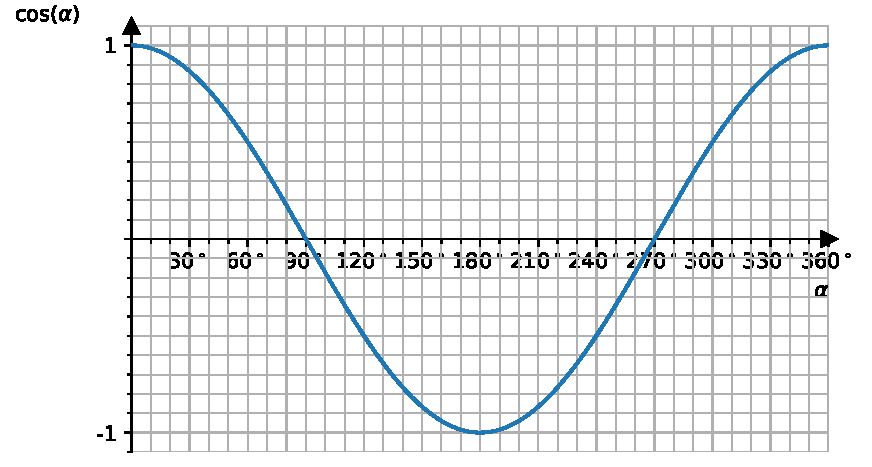
\includegraphics{7_Trigonometrische_Funktionen_files/figure-pdf/cell-3-output-1.pdf}

\begin{tcolorbox}[enhanced jigsaw, colbacktitle=quarto-callout-note-color!10!white, breakable, bottomtitle=1mm, toptitle=1mm, opacitybacktitle=0.6, opacityback=0, rightrule=.15mm, titlerule=0mm, leftrule=.75mm, colframe=quarto-callout-note-color-frame, toprule=.15mm, left=2mm, colback=white, title=\textcolor{quarto-callout-note-color}{\faInfo}\hspace{0.5em}{Definition: Tangens-Funktion im Dreieck}, coltitle=black, arc=.35mm, bottomrule=.15mm]

Gegeben:

\begin{itemize}
\tightlist
\item
  rechtwinkliges Dreieck ABC
\end{itemize}

Die Abbildung, die jeder Winkelgröße den Tangens zum Winkel im
zugehörigen rechtwinkligen Dreieck zuordnet, heißt
\textbf{Tangensfunktion}

\end{tcolorbox}

\textbf{Funktionsgraph der Tangens-Funktion:}

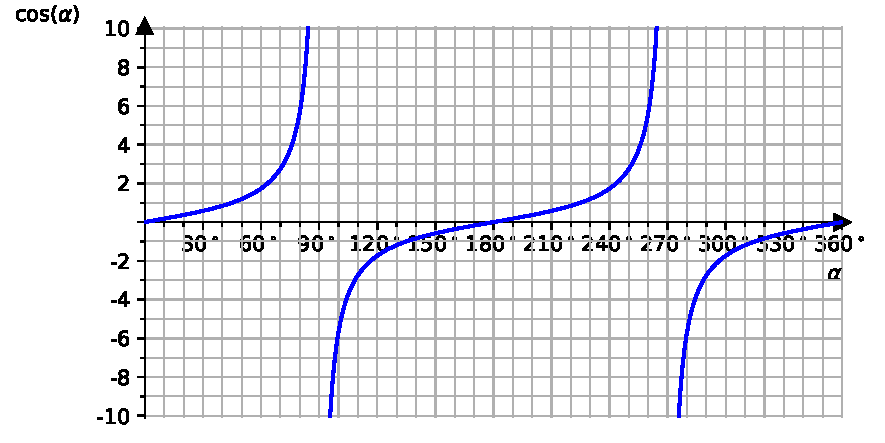
\includegraphics{7_Trigonometrische_Funktionen_files/figure-pdf/cell-4-output-1.pdf}

\subsubsection{7.2 reelwertige
Winkelfunktionen}\label{reelwertige-winkelfunktionen}

\paragraph{Bogenmaß}\label{bogenmauxdf}

\begin{figure}[H]

{\centering \includegraphics[width=2.08333in,height=\textheight]{/Users/martin/Workspace/Jupyter_Notebooks/Mathe_KS/1_Analysis/4_Zusammenhang_Funktion_Graph/images/6bogenmaß.jpg}

}

\caption{Einheitskreis}

\end{figure}%

\textbf{Beobachtung:}

\begin{itemize}
\tightlist
\item
  Jedem Winkel kann eindeutig eine Kreisbogenlänge zugeordnet werden.
\item
  Diese Zuordnung ist bijektiv.
\item
  Die Kreisbogenlänge ist eine reelle Zahl.
\end{itemize}

\begin{tcolorbox}[enhanced jigsaw, colbacktitle=quarto-callout-important-color!10!white, breakable, bottomtitle=1mm, toptitle=1mm, opacitybacktitle=0.6, opacityback=0, rightrule=.15mm, titlerule=0mm, leftrule=.75mm, colframe=quarto-callout-important-color-frame, toprule=.15mm, left=2mm, colback=white, title=\textcolor{quarto-callout-important-color}{\faExclamation}\hspace{0.5em}{Satz:}, coltitle=black, arc=.35mm, bottomrule=.15mm]

Gegeben: - Kreis \(k(M;r)\) mit Mittelpunkt \(M\) und Radius \(r\) -
Kreissektor mit Öffnungswinkelswinkel \(\alpha\)

Die Kreisbogenlänge \(b\) des Kreissegments (Bogenmaß) wird berechnet
mit: \[
 b= r \cdot \frac{\pi \cdot\alpha}{180^\circ}
\]

\end{tcolorbox}

\subparagraph{Folgerung}\label{folgerung}

Damit lässt sich wie folgt auch zu jeder reelen Zahl \(x\) ein Wert
\(\sin(x), \cos(x)\) bzw. \(\tan(x)\) zuordnen: \[
\begin{aligned}
&\alpha &\rightarrow & \sin(\alpha) \\
& \downarrow & &= \\
&x &\rightarrow &\sin(x)
\end{aligned}
\]

\subparagraph{Funktionsterme}\label{funktionsterme}

Zuordnung Winkel \(\rightarrow\) Bogenlänge \[
g(\alpha)=\left(r \cdot \frac{\pi \cdot\alpha}{180^\circ}\right)
\] Zuordnung Bogenlänge (reele Zahl) \(\rightarrow\) Sinus \[
f(x)=f(g(\alpha))=\sin\left(r \cdot \frac{\pi \cdot\alpha}{180^\circ}\right)=\sin(x)
\]

\paragraph{Winkelfunktionen}\label{winkelfunktionen}

\subparagraph{Sinus-Funktion}\label{sinus-funktion}

\begin{itemize}
\tightlist
\item
  Defintionsmenge: \(\mathbb{R}\)
\item
  Wertemenge: \(W=\{f(x)|-1\leq f(x)\leq 1\}\)
\item
  periodisch
\item
  Periode \(p=2\pi\)
\item
  punktsymmetrisch zum Ursprung
\end{itemize}

\[
\sin(-x)=-\sin(x)
\]

\begin{itemize}
\tightlist
\item
  Nullstellen:
\end{itemize}

\[
\begin{aligned}
..., -\pi, 0, \pi, 2\pi, 3\pi, ...\\
\text{allgemein: }k\cdot \pi \quad, k\in \mathbb{Z}
\end{aligned}
\]

\begin{itemize}
\tightlist
\item
  Maximalstellen:
\end{itemize}

\[
\begin{aligned}
..., -\frac{3}{2}\pi, \frac{\pi}{2}, \frac{5}{2}\pi, \frac{9}{2}\pi, ...\\
\text{allgemein: }\frac{\pi}{2}+k\cdot 2\pi \quad , k\in \mathbb{Z}
\end{aligned}
\]

\begin{itemize}
\tightlist
\item
  Minimalstellen:
\end{itemize}

\[
\begin{aligned}
..., -\frac{5}{2}\pi, -\frac{\pi}{2}, \frac{3}{2}\pi, \frac{7}{2}\pi, ...\\
\text{allgemein: }\frac{3}{2}\pi + k\cdot 2\pi \quad ,k\in \mathbb{Z}
\end{aligned}
\]

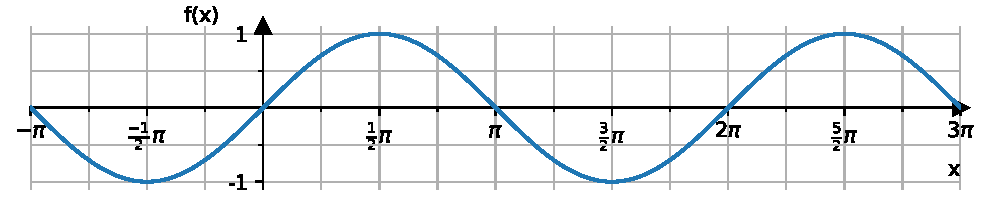
\includegraphics{7_Trigonometrische_Funktionen_files/figure-pdf/cell-5-output-1.pdf}

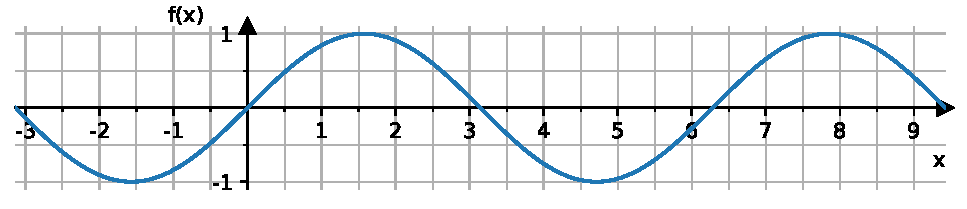
\includegraphics{7_Trigonometrische_Funktionen_files/figure-pdf/cell-6-output-1.pdf}

\subparagraph{Kosinus-Funktion}\label{kosinus-funktion}

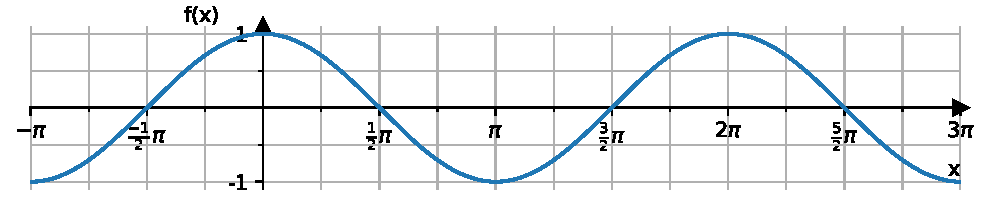
\includegraphics{7_Trigonometrische_Funktionen_files/figure-pdf/cell-7-output-1.pdf}

\textbf{Eigenschaften:}

\begin{itemize}
\tightlist
\item
  Defintionsmenge: \(\mathbb{R}\)
\item
  Wertemenge: \(W=\{f(x)|-1\leq f(x)\leq 1\}\)
\item
  periodisch
\item
  Periode \(p=2\pi\)
\item
  achsensymmetrisch zur y-Achse
\end{itemize}

\[
\cos(-x)=\cos(x)
\]

\begin{itemize}
\tightlist
\item
  Nullstellen:
\end{itemize}

\[
\begin{aligned}
..., -\frac{\pi}{2}, \frac{\pi}{2}, \frac{3}{2}\pi, \frac{5}{2}\pi, ...\\
\text{allgemein: }\frac{2k+1}{2}\cdot \pi \quad ,k\in \mathbb{Z}
\end{aligned}
\]

\begin{itemize}
\tightlist
\item
  Maximalstellen:
\end{itemize}

\[
\begin{aligned}
..., -2\pi, 0, 2\pi, 4\pi, ...\\
\text{allgemein: }2k\cdot \pi  \quad ,k\in \mathbb{Z}
\end{aligned}
\]

\begin{itemize}
\tightlist
\item
  Minimalstellen:
\end{itemize}

\[
\begin{aligned}
..., -\pi, \pi, 3\pi, 5\pi, ...\\
\text{allgemein: }(2k+1)\pi \quad , k\in \mathbb{Z}
\end{aligned}
\]

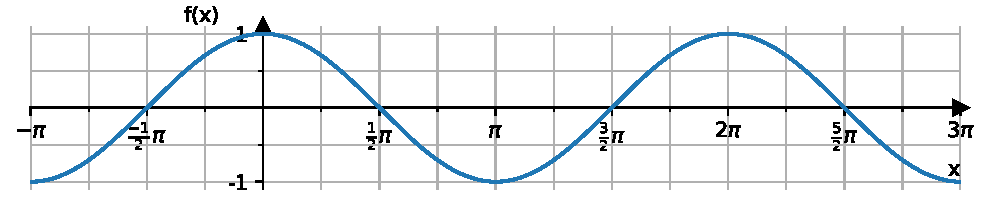
\includegraphics{7_Trigonometrische_Funktionen_files/figure-pdf/cell-8-output-1.pdf}

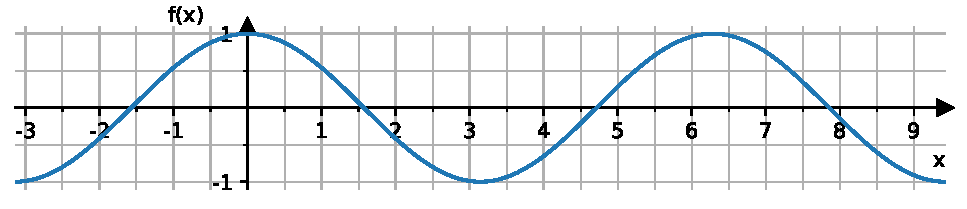
\includegraphics{7_Trigonometrische_Funktionen_files/figure-pdf/cell-9-output-1.pdf}

\paragraph{Verschieben der Sinusfunktion entlang der
y-Achse}\label{verschieben-der-sinusfunktion-entlang-der-y-achse}

Funktionsgleichung:

\[
f(x)=\sin(x)+d
\]

Die Mittellinie ist die Gerade \(y=d\)

\subparagraph{Beispiel}\label{beispiel}

\[
f(x)= \sin(x)-2
\]

Mittellinie: \(y=-2\)

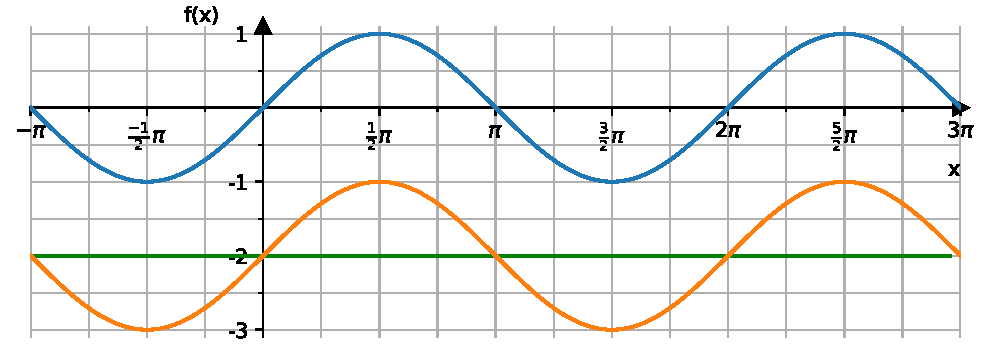
\includegraphics{7_Trigonometrische_Funktionen_files/figure-pdf/cell-10-output-1.pdf}

\subparagraph{Verschieben entlang der
x-Achse}\label{verschieben-entlang-der-x-achse}

Funktionsgleichung:

\[
f(x)=\sin(x-c)
\]

Man nennt \(c\) auch Phase.

\subparagraph{Beipsiel}\label{beipsiel}

\[
f(x)= \sin(x-1)
\]

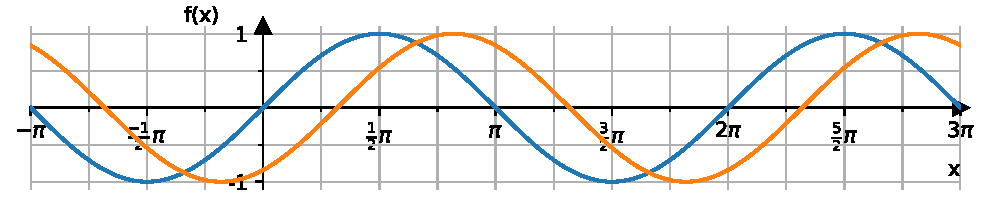
\includegraphics{7_Trigonometrische_Funktionen_files/figure-pdf/cell-11-output-1.pdf}

\subparagraph{Beobachtung}\label{beobachtung}

\[
f(x)=\sin(x-\left(-\frac{1}{2}\cdot \pi\right))=\cos(x)
\]

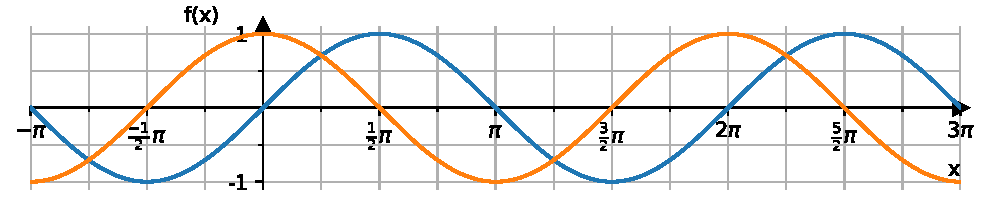
\includegraphics{7_Trigonometrische_Funktionen_files/figure-pdf/cell-12-output-1.pdf}

\subparagraph{Strecken / Stauchen}\label{strecken-stauchen}

Funktionsgleichung: \[
f(x)=a\cdot \sin(x)
\] \(|a|\) nennt man Amplitude (= Ausschlag). Die Amplitude ist immer
positiv.

\subparagraph{Beipsiel}\label{beipsiel-1}

\[
f(x)= 3\cdot \sin(x)
\]

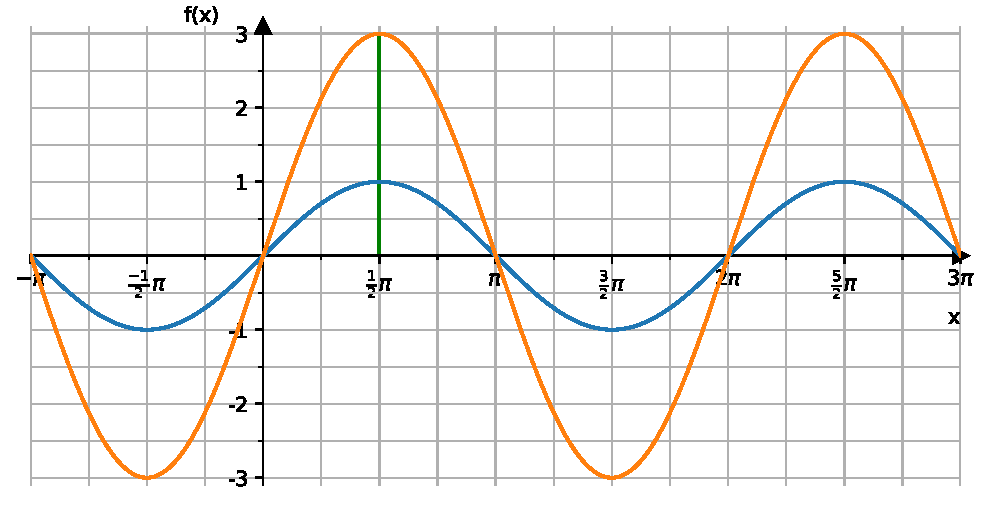
\includegraphics{7_Trigonometrische_Funktionen_files/figure-pdf/cell-13-output-1.pdf}

\subparagraph{Periode verändern}\label{periode-veruxe4ndern}

Funktionsgleichung:

\[
f(x)=\sin(b\cdot x)
\]

Das Verhältnis \[
p=\frac{2\pi}{b}
\] nennt man Periode.

\subparagraph{Beispiel}\label{beispiel-1}

\[
f(x)= \sin(2\cdot x)
\]

Die Periode ist: \[
p = \frac{2 \pi}{2}=\pi
\]

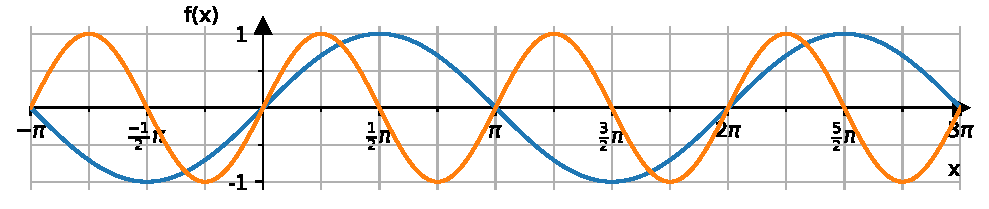
\includegraphics{7_Trigonometrische_Funktionen_files/figure-pdf/cell-14-output-1.pdf}

\subparagraph{Beispiel}\label{beispiel-2}

\[
f(x)= \sin\left(\frac{1}{3}\cdot x\right)
\]

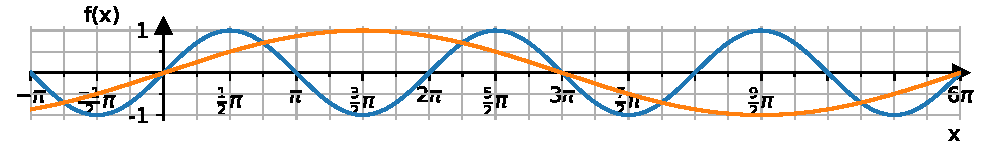
\includegraphics{7_Trigonometrische_Funktionen_files/figure-pdf/cell-15-output-1.pdf}

\subparagraph{Spiegeln an der x-Achse}\label{spiegeln-an-der-x-achse}

Funktionsgleichung: \[
f(x)=-\sin(x) = \sin(-x)
\]

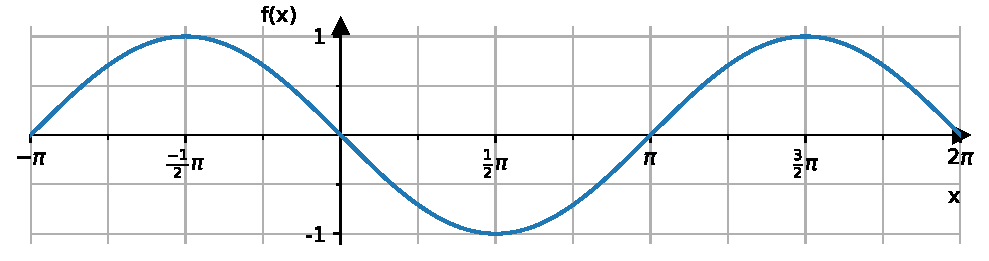
\includegraphics{7_Trigonometrische_Funktionen_files/figure-pdf/cell-16-output-1.pdf}

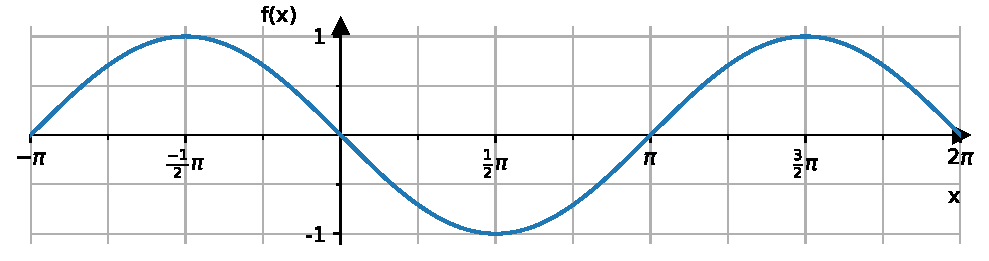
\includegraphics{7_Trigonometrische_Funktionen_files/figure-pdf/cell-17-output-1.pdf}

\subparagraph{Allgemeine
Sinus-Funktion}\label{allgemeine-sinus-funktion}

\begin{tcolorbox}[enhanced jigsaw, colbacktitle=quarto-callout-note-color!10!white, breakable, bottomtitle=1mm, toptitle=1mm, opacitybacktitle=0.6, opacityback=0, rightrule=.15mm, titlerule=0mm, leftrule=.75mm, colframe=quarto-callout-note-color-frame, toprule=.15mm, left=2mm, colback=white, title=\textcolor{quarto-callout-note-color}{\faInfo}\hspace{0.5em}{Definition}, coltitle=black, arc=.35mm, bottomrule=.15mm]

\(a, b, c, d \in \mathbb{R}\) Der Graph der Funktion\\
\[
g(x)=a\cdot \sin(b(x-c))+d
\] geht aus der Funktion \[
f(x) = \sin(x)
\] hervor, indem - f um \(|a|\) in y-Richtung gestreckt wird. Die
Amplitude A entspricht \(A = |a|\)\\
- f um Faktor \(\frac{1}{b}\) in x-Richtung gestreckt wird.\\
- f um c in x-Richtung und um d in y-Richtung verschoben wird.

\end{tcolorbox}

\begin{tcolorbox}[enhanced jigsaw, colbacktitle=quarto-callout-tip-color!10!white, breakable, bottomtitle=1mm, toptitle=1mm, opacitybacktitle=0.6, opacityback=0, rightrule=.15mm, titlerule=0mm, leftrule=.75mm, colframe=quarto-callout-tip-color-frame, toprule=.15mm, left=2mm, colback=white, title=\textcolor{quarto-callout-tip-color}{\faLightbulb}\hspace{0.5em}{Bemerkung}, coltitle=black, arc=.35mm, bottomrule=.15mm]

Analoge Aussagen gelten auch für die Kosinus-Funktion.

Der Graph der Kosinus-Funktion geht aus dem Graph der Sinus-Funktion
durch Verschiebung in x-Richtung um \(-\frac{\pi}{2}\) hervor.

\end{tcolorbox}

\subparagraph{Beispiel:}\label{beispiel-3}

\(a=5\)\\
\(b=2\)\\
\(c=-2\)\\
\(d=-1\)

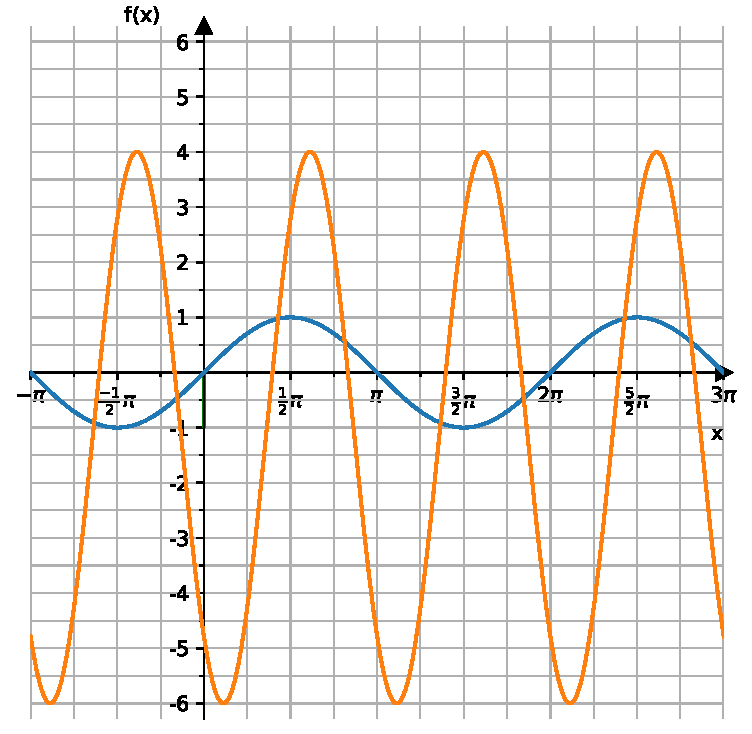
\includegraphics{7_Trigonometrische_Funktionen_files/figure-pdf/cell-18-output-1.pdf}



\end{document}
